\chapter{Implementation}
How a prototype implementation could be realised by applying the above outlined concepts and architectures will be discussed in this section. This implementation or more accurately, pseudo code, will give a broad overview of what can be derived translated from the concept into the software, by discussing the key elements. All these descriptions are so far known 'best practice', but do not tackle all software-architectural concerns of the FBP as long as the concept and consensus is not violated.
\section{Contracts}
Implementing the contracts in a prototype implementation is significantly easier than it would be for a real-world application. As mentioned above, it consists of the knowledge of each other and where they are located.
\begin{figure}
    
    \begin{center}
        \begin{tabular}{llll} \toprule
            Client-Contract&value&ISP-contract&value\\ \midrule
            actual public key:& cli001 &  actual public key: &isp001  \\ 
            actual private key:& ****** & actual private key:& ****** \\
            Client-ISP feed ID:& cli001\_isp001 &ISP-Client feed ID:&isp001\_cli001 \\ 
            ISP public key&isp001&Client public key:&cli001\\
            ISP-Client feed ID&isp001\_cli001&Client-ISP feed ID:&cli001\_isp001\\
            ISP location:&131.152.158.21:5000 &Client location:& 131.152.211.12:5000 \\\bottomrule
        \end{tabular}
    \end{center}
    \caption{The client's and the ISP's contract.}
\end{figure}

In this table we can see a basic contract with all the information needed. This contract can be broken down even more, since the feed-IDs are just appended public keys. In the public and private key fields a first abstraction to the real-world application is made, the public and private keys would most likely be some 256-bits long integer key pairs for example Curve25519 [\citenum{hankerson2006guide}]. This would result in a 64 digit long hexadecimal representation. The terms here act as simplification and easier distinguishable keys. Having this setup for example with a Curve25519 key pair, it is best practice to store them in a secrets or key file. Therefore the most basic contract can look like this:

\begin{figure}
    
    \begin{center}  
        \begin{tabular}{llll} \toprule
            Client-Contract&value&ISP-contract&value\\ \midrule
            key file:& cli001.key &  key file: &isp001.key  \\ 
            ISP public key&isp001&Client public key:&cli001\\
            ISP location:&.\slash isp001\slash &Client location:& .\slash cli001\slash \\\bottomrule
        \end{tabular}  
    \end{center}
    \caption{A more simplified contract.}
\end{figure}
This even more simplified base, which runs on a localhost over the file system, can be stored in any suitable file type and the rest of the contract, such as the feed-IDs can be built by the program, if the rules are defined over the entire network. These contracts must be stored somewhere in the software, but the implementation can be freely chosen.

\section{Replicated Feeds}
This implementation was developed by Prof. Dr. Christian Tschudin [\citenum{entropy}]. It is a very simplified version of an append-only log in the .pcap format, generated from a Curve25519 key pair. Every log entry is signed by some private key, which leads to integrity, but not security. The entire security aspect was omitted from this thesis.
\subsection{Structure}
The Feed is a list of log entries. Each log entry consists of three main parts: meta data, the signature and the content. The meta data holds the information about the current log entry, such as the feed-ID of its feed, its sequence number, which is the internal position of the log entry in the feed, a hash reference to the log entry before and its own hash value of the content for the next log entry to reference. Next comes the signature, which signs the meta data. The content part is what is actually put into the log entry. Since all the information is stored in the CBOR [\citenum{bormann2013concise}] format and held in a pcap file, the result is a binary array which holds important properties useful for the bundling. Either a new log entry can be written with a key or an existing log entry can be appended to the binary array without validation. This mechanism is a key feature for the bundling aspect.
\subsection{Replication}
The replication mechanism is invoked after each write operation to a feed. Generally speaking, this could be realised easily with TCP or UDP in a real network. Since this basic implementation has no connection to the internet, it replicates feeds in the file system. This was solved by simply copying the feed to the corresponding folder given in the contract.
\section{RPC}
Having the contract and replicated feeds, the type of RPC-protocol has its turn. To communicate between two participants, four general methods are needed as listed below. By having a simple serialisable data structure for requests and results, it is easy to incorporate them into the feeds. Requests call services, which use the given attributes and produce a result, as advanced in the original RPC-protocol by \citet{birrell1984implementing}.
\section{Data Structure}
A suitable data structure or format is a dictionary or a JSON-String, having keys that reference a field, as well as being serialisable. In this structure, an ID must be given to distinguish repeated requests, as well as map the results to their request, a type has to be set to distinguish request and result, further the service to be called is needed as well as the attributes or the result of the call. This results in a minimal set of keys for request and result:\\

    \begin{python}
        \begin{lstlisting}
            request = {'ID':0, 'type':'request', 'service':'echo', 
            'attributes':['An echo']}
            result = {'ID':0, 'type':'result', 'result':'An echo'}
        \end{lstlisting}
    \end{python}
    



Having the ID as an identifier, the caller can look up the request made and map the result to the call.
\section{Services}
Services are the procedures called by the caller and executed by the callee. In the feed bundle protocol there are some key services which have to be considered:
\begin{itemize}
    \item \lstinline{echo} - It just returns the given attributes.
    \item \lstinline{get_service_catalog} - The caller needs a list of all services the caller has available.
    \item \lstinline{introduce} - This service passes a request to the server specified in the attributes and introduces the caller(client) to it and signs a contract.
    \item \lstinline{detruce} - This closes an previously established contract and erases all information built on it.
    \item \lstinline{get_servers} - A list of servers is needed to call the introduce service. Since the caller has no knowledge of servers, this is essential.
\end{itemize}
\section{API}
As a disclaimer, these API methods correspond only to the logical aspect of the pseudo code. There are many ways to implement them in differing software-architecturial styles, the implementation only shows what is minimally needed and executed.
\subsection{Send Request}
The \lstinline{send_request()} method needs to have knowledge of the service to be invoke and its attributes, as well as a destination. As described above, it is not a "sending" in the old-fashioned way, the destination corresponds to the Caller-Callee feed where the caller is the source and the Callee is the destination. Given these parameters, a request can be formed and written to the destination feed, whereby the feed must be replicated afterwards.
\begin{python}
    \lstinputlisting[]{Code/send_request.py}
    
\end{python}

 
\subsection{Read Request}
This method needs to follow on a detected feed change. This can be realised either by a global polling mechanism, which invokes the \lstinline{read_request()} method, or directly in the method by listening to a feed. It takes the request, extracts its contents and invokes the specified service and waits for its result. Afterwards, it either returns the result or passes it directly to the \lstinline{send_result()} method. 
\begin{python}
    \lstinputlisting[]{Code/read_request.py}
    
\end{python}


\subsection{Send Result}
This method is very similar to the \lstinline{send_request()} method. It uses the previously executed request to gain information about the ID, forms the result and writes it to the Callee-Caller feed.
\begin{python}
\lstinputlisting[]{Code/send_result.py}
    
\end{python}

\subsection{Read Result}
This method also to follows on a detected feed change, takes the result and closes the request. Due to the fact that quite some time has elapsed since the \lstinline{send_request()} method, there is also a threading issue. Whether the \lstinline{send_request()} method is blocking or not depends on the overlay of the FBP and cannot be decided in general, although it is blocking in the implementation of \citet{birrell1984implementing}. Therefore, it needs to be taken into account, but not considered at this API level.
\begin{python}
\lstinputlisting[]{Code/read_result.py}
    
\end{python}


\section{Bundling}
Leading to the bundling key element, the other components were laid out and specifically designed for this. Two approaches to bundling can be made. One consists of a single feed-pair between ISP and the server where all the communication happens, the other involves two feed-pairs where one acts only for request from the ISP to the server and the other only for multiplexed client requests. In this section, the first approach is discussed, since they do not differ significantly.
\subsection{Introducing and Detrucing}
\begin{figure}
    \centering
    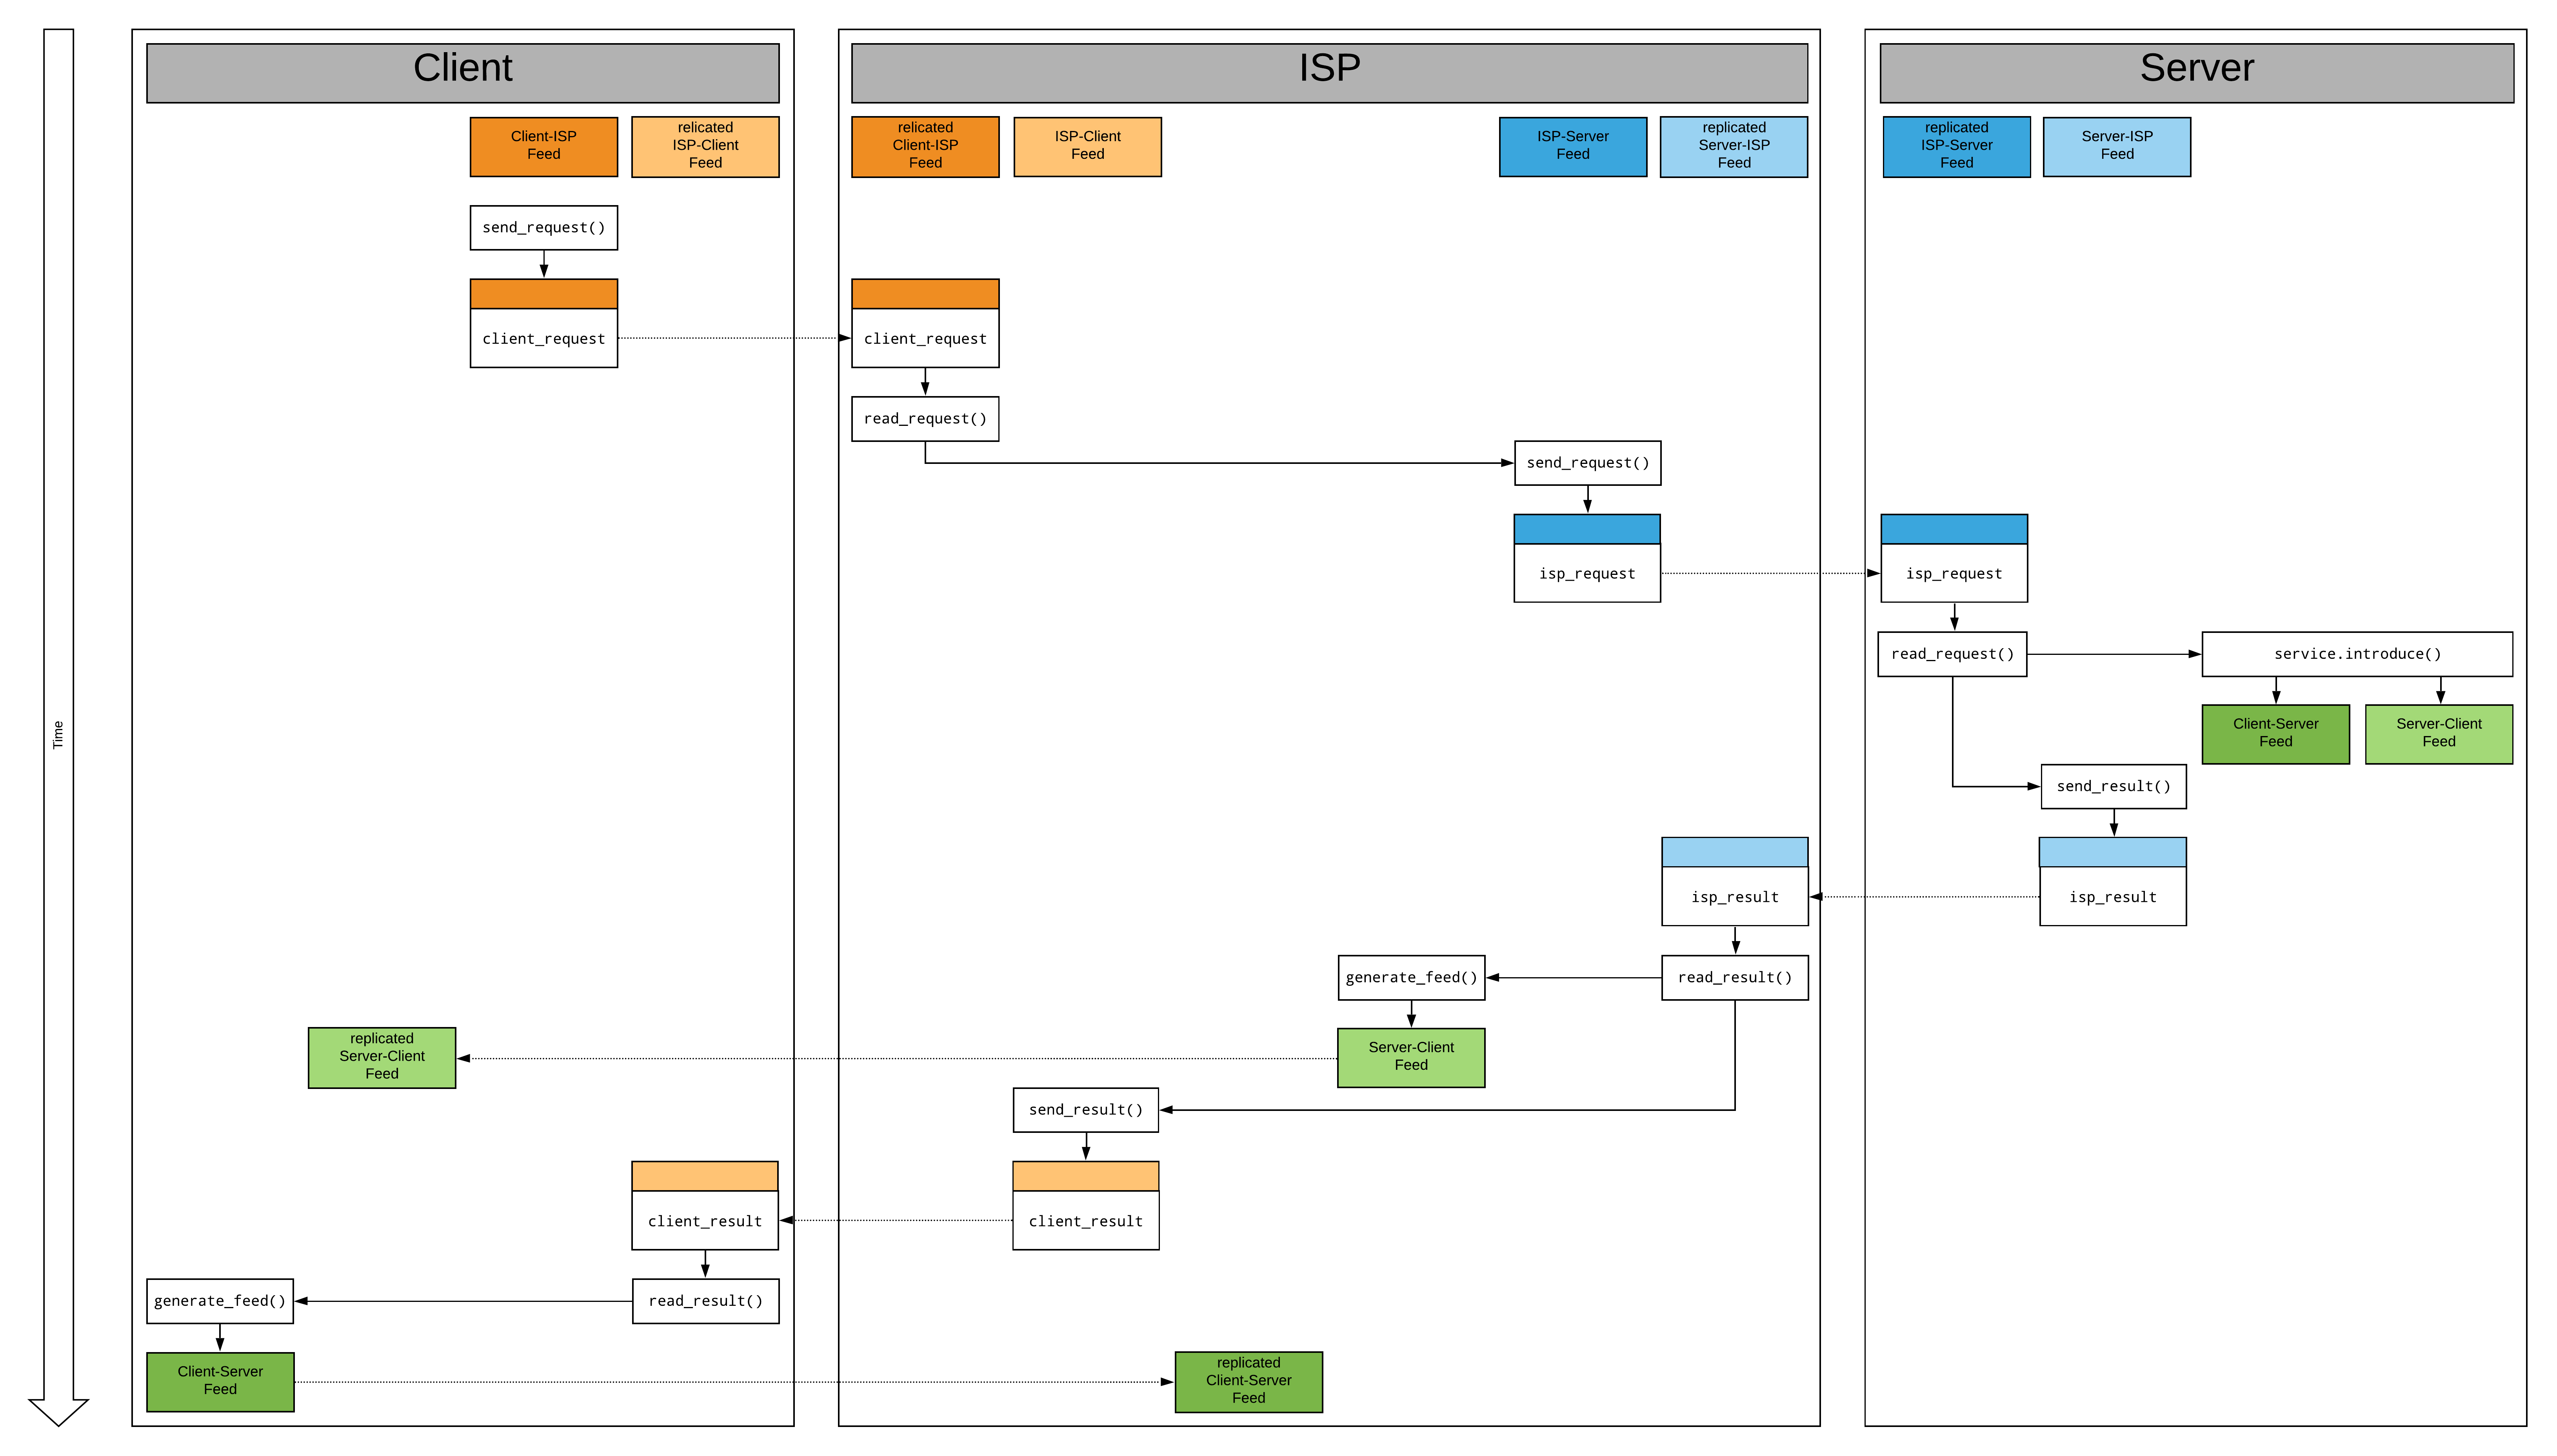
\includegraphics[width=\textwidth]{full_rpc}
    \caption{A full RPC-request for the introduce-service}
    \label{fig:fullprc}
\end{figure}

As seen in the RPC implementation, a client calls the introduce-service with the server it wants to be introduced to. At this point, the ISP holds a request from the client. The ISP does an RPC-request by itself to the server as followed:
\\
\begin{python}
    
\begin{lstlisting}
client_request = {'ID':0, 'type':'request', 'service':'introduce', 
                  'attributes':'ser001'}
\end{lstlisting}
\begin{lstlisting}
isp_request = {'ID':0, 'client_request_ID':0, 'type':'request', 
               'service':'introduce', 'attributes':{'public_key':'cli001'}}
\end{lstlisting}
\end{python}


In this request, everything the server needs to know is given. After creating the entire feed-pair and setting up the contract, the result is returned to the ISP.
\\
\begin{python}
    
\begin{lstlisting}
isp_result = {'ID':0, 'client_request_ID':0, 'type':'result', 
              'result':{'public_key':'ser001', 
                        'client_server_feed_ID':'cli001_ser001',
                        'server_client_feed_ID':'ser001_cli001'
                        }
             }
\end{lstlisting}
\end{python}

With this information, the ISP can build the Server-Client feed and replicate it, since the location of the client is already known.
Afterwards, the client receives their result on the initial introduce-request and can build the Client-Server feed and replicate it to the ISP.\\
\begin{python}
    
\begin{lstlisting}
client_result = {'ID':0, 'type':'result', 
                 'result':{'public_key':'ser001', 
                           'client_server_feed_ID':'cli001_ser001', 
                           'server_client_feed_ID':'ser001_cli001'
                          }
                 }
\end{lstlisting}
\end{python}

This implementation corresponds to a client, ISP and server, which do not know how the other labels their feeds, nor over which public key the connection will be handled. This lays the base for several ISP nodes discussed in the Future Work Section. 


\subsection{Multiplexing}
Having now an introduced client we need to have a look at the communication between it and the server. As previously mentioned, there is no direct feed replication between the client and the server over the ISP. Instead the requests are taken from the Client-Server feed at the ISP and multiplexed into the ISP-Server feed. Afterwards, this same request is demultiplexed from the replication of the ISP-Server feed in the server and transferred to the Client-Server feed representation in the server.\\
In order to achieve this, a new type is accepted and a new field is added in the RPC-data structure: the mux-type and the meta-field. Here an abstraction of the structure of a ’mux-request’:\\
\begin{python}
    
\begin{lstlisting}
mux_request = {'ID':1, 'type':'mux', 
               'meta':{'feed_ID':'cli001_ser001'},
               'client_request':{'ID':1, 'type':'request', 'service':'echo', 
                                 'attributes':'hello server'}
              }
\end{lstlisting}
\end{python}

The mux type ensures that the log entry is not designed for the read result method of the RPC and all additional information needed by the server is given in the meta field. Any server reading this knows in which feed the request belongs and writes it into this feed and performs the requested service form there. The result is written in the Server-ISP feed as followed:\\
\begin{python}
    
\begin{lstlisting}
mux_result = {'ID':1, 'type':'mux', 
              'meta':{'feed_ID':'ser001_cli001'},
              'client_result':{'ID':1, 'type':'result', 'result':'hello server'}
             }
\end{lstlisting}
\end{python}

Again, the meta data describes how to handle this specific mux-result in the ISP. If we approach the problem like this, one particular inconsistency occurs. When writing in feeds with this approach, the signing process is violated and the integrity broken. Hence the replicated feed offers a solution for this. Instead of extracting the request, and then rewriting it, the whole log entry is put as the value of the key request or result and at demultiplexing stage appended bytewise to the corresponding feed.\\
\begin{figure}
    \centering
    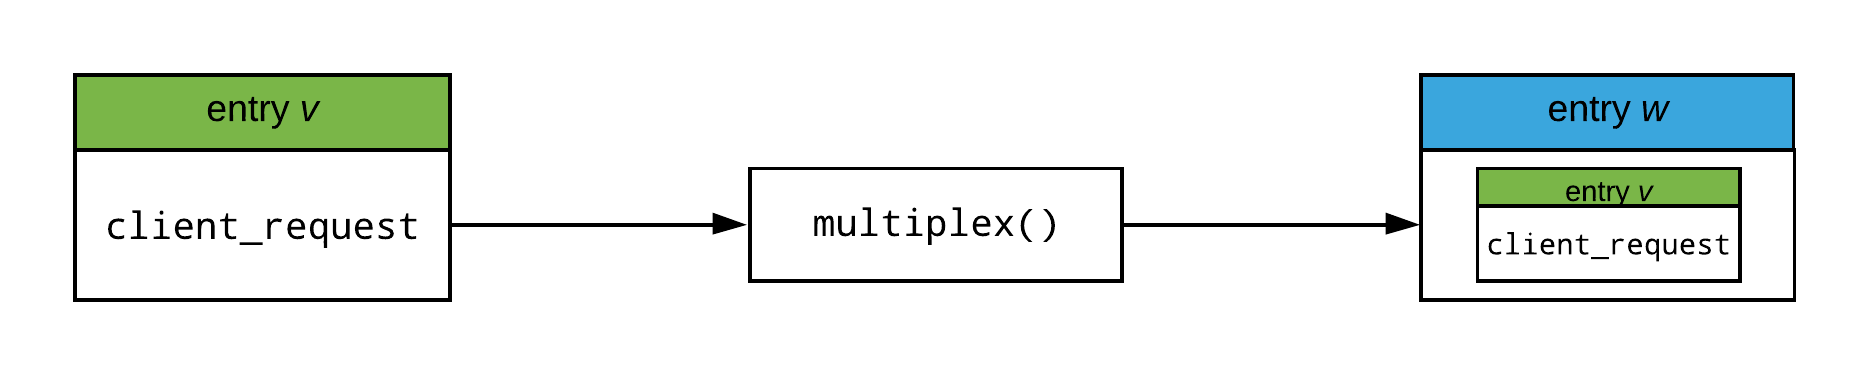
\includegraphics[width=0.7\textwidth]{simple_mux}
    %\caption{Log entry $v$ gets multiplexed in log entry $w$}
    \label{fig:simplemux}
\end{figure}


Clearly seen is the full log entry $v$ of the Client-Server feed. By putting $v$ directly in the log entry $w$ of the ISP-Server feed no information gets lost or changed. This ensures integrity and replicates the feed exactly as it is: bytewise over the ISP to the server. 
\begin{figure}
    \centering
    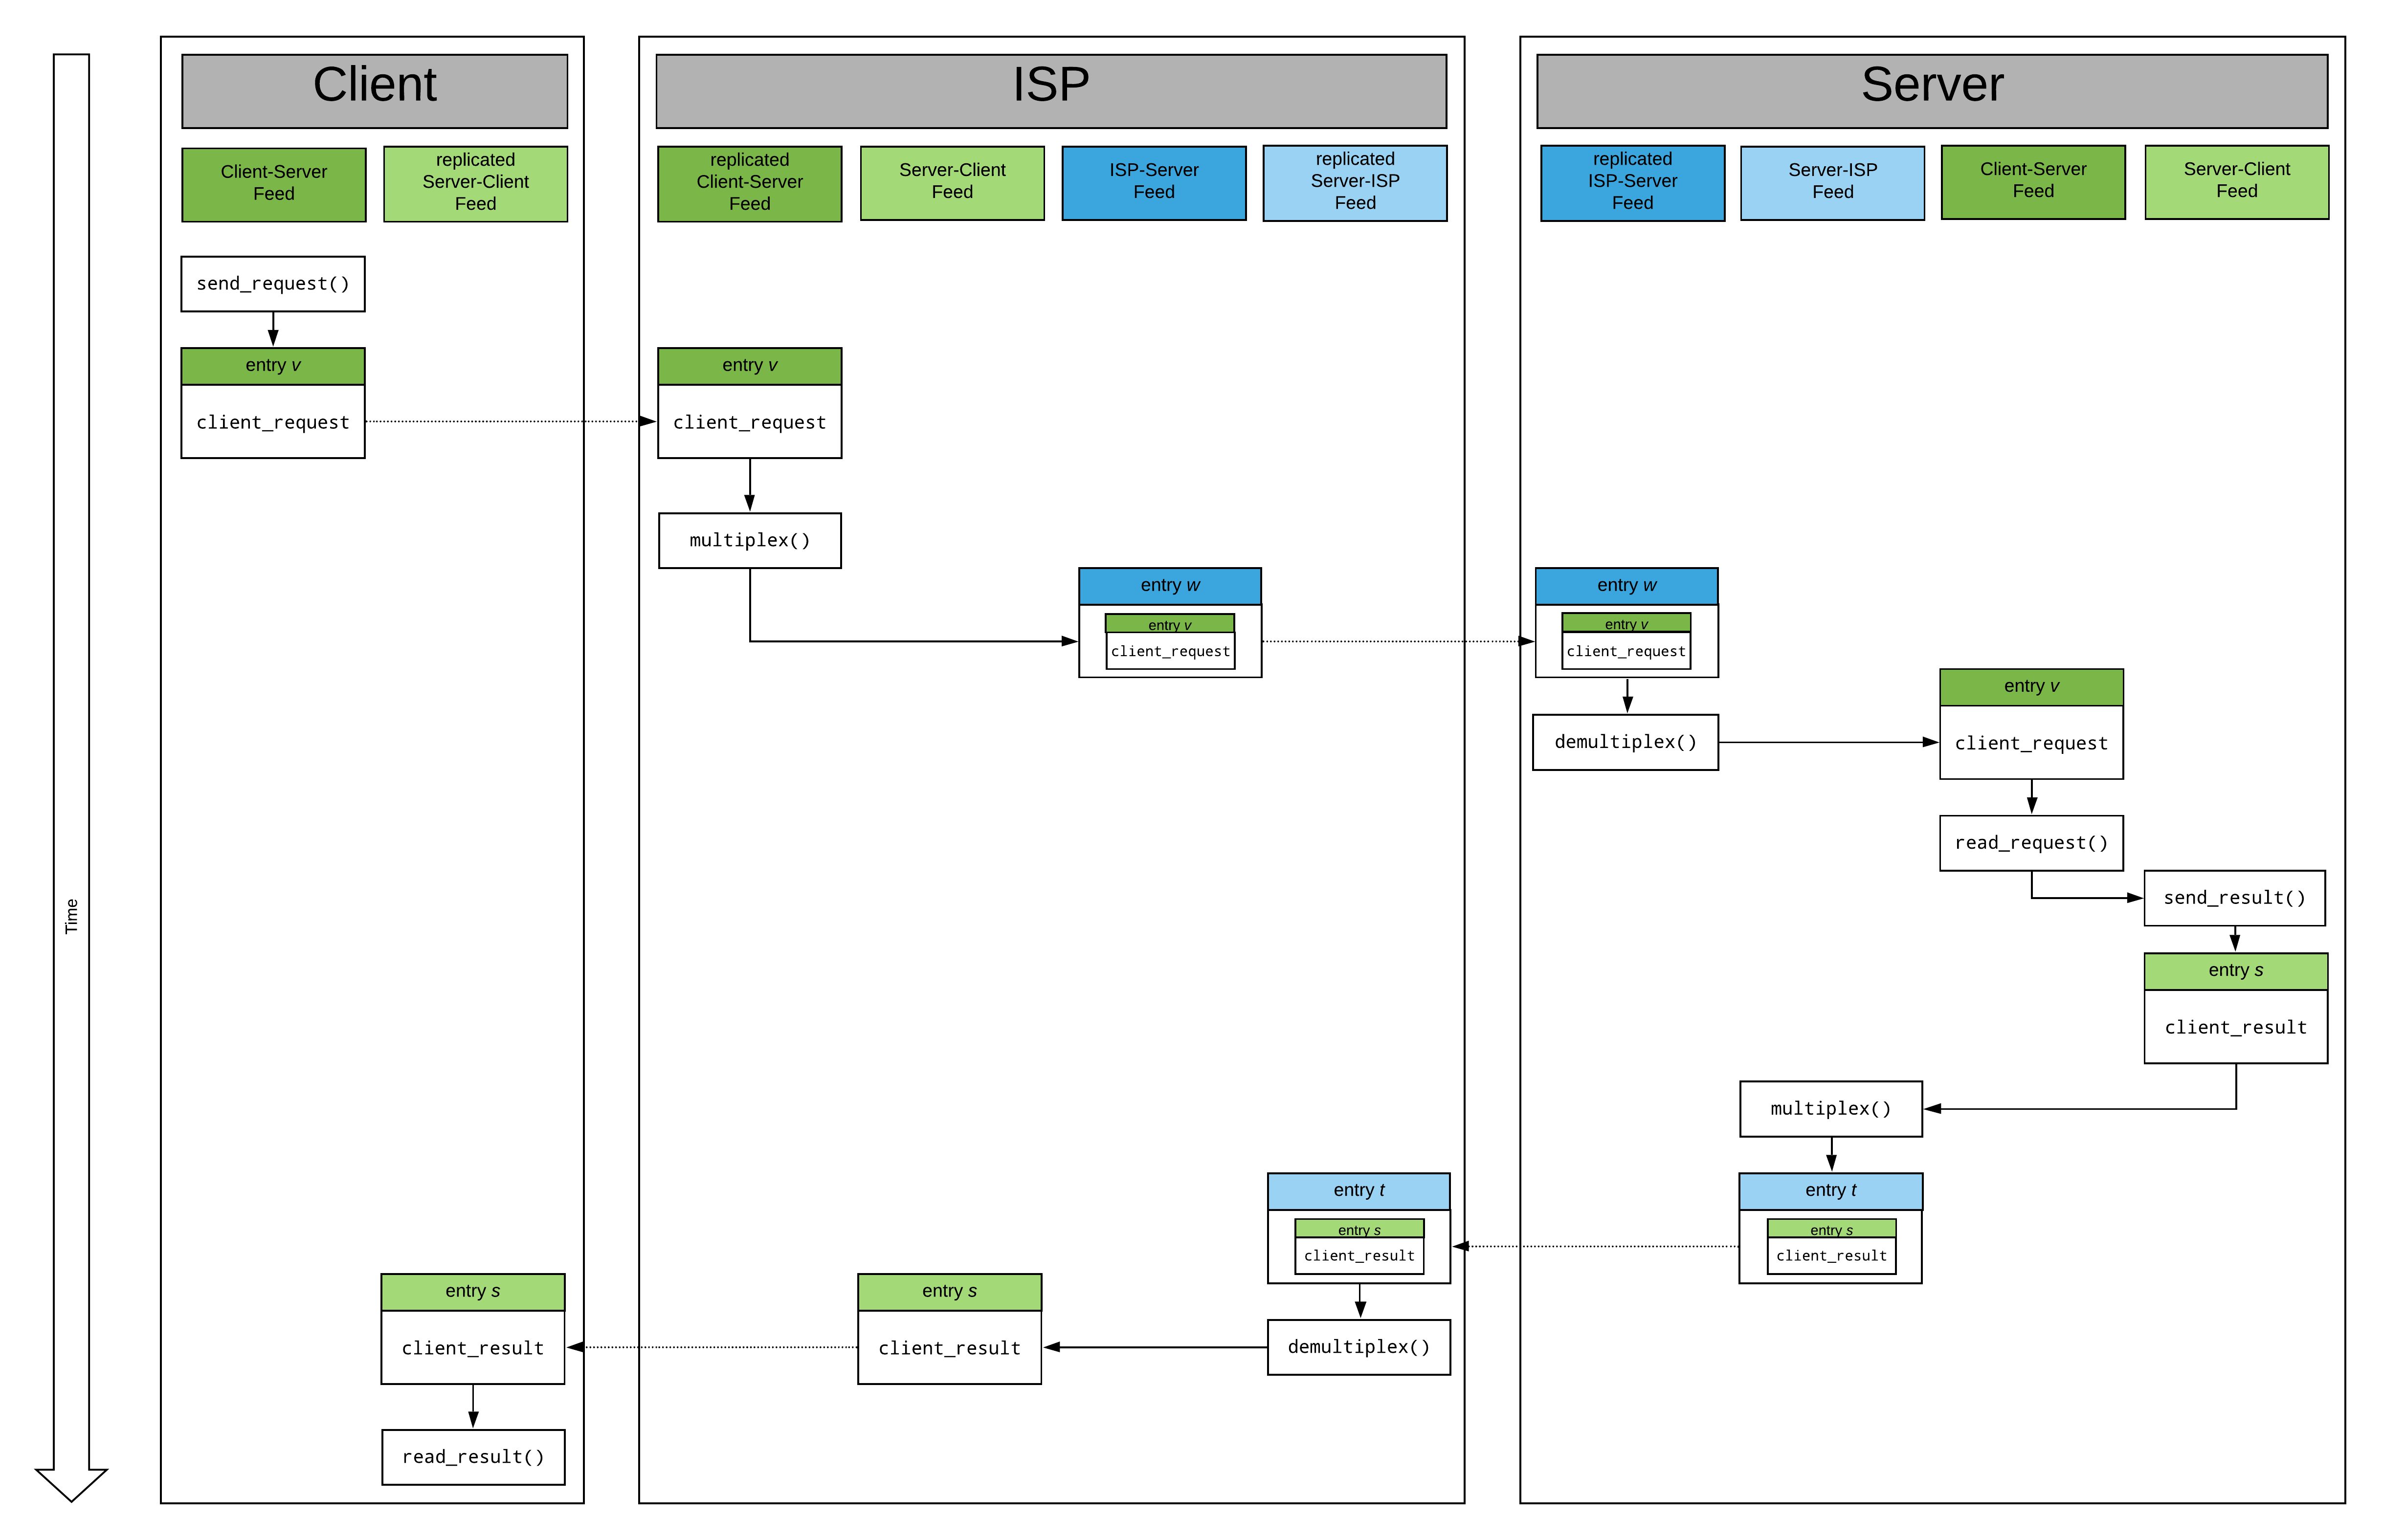
\includegraphics[width=\textwidth]{full_mux}
    \caption{A full multiplexed RPC-request from client to server}
    \label{fig:fullmux}
\end{figure}